\ifthenelse{\boolean{acl}}{
\section{Additional Background on Federated Learning (FL) with Differential Privacy (DP)} \label{app:background}
\subsection{DP Formulation} \label{subsec:dp_def}
We present the definition of ($\epsilon$, $\delta$)-DP~\citep{dwork2006calibrating,dwork2014algorithmic} to quantify the privacy protection. 
\begin{definition}[$(\epsilon,\delta)$-Differential Privacy]
  A randomized algorithm $\mathcal{M}$ satisfies  ($\epsilon$, $\delta$)-DP for $\mathbb{D}$ if for any two neighboring datasets $\mathbb{D}$, $\mathbb{D}'$ and for all $\mathcal{S}\subset \text{Range}(\mathcal{M})$: 
\[
\textstyle{\Pr[\mathcal{M}(\mathbb{D}) \in \mathcal{S}] \leq e^{\epsilon}\Pr[\mathcal{M}(\mathbb{D}') \in \mathcal{S}] +\delta}
.\]
\end{definition}
Smaller ($\epsilon$, $\delta$) values suggest stronger DP guarantees, and we often measure $\epsilon$ at a fixed small $\delta=10^{-10}$. DP-FTRL also uses an alternative definition, $\rho$-zCDP (zero-Concentrated DP)~\citep{bun2016concentrated} designed for Gaussian mechanism, and smaller $\rho$ suggests stronger DP guarantees. We use PLD (privacy Loss Distributions) accounting~\citep{doroshenko2022connect,pldlib} to convert $\rho$-zCDP to ($\epsilon$, $\delta$) DP. When applying DP in FL, the neighboring datasets $\mathbb{D}$, $\mathbb{D}'$ are defined by zeroing out the contribution of all data on a user device. More discussions on neighboring dataset for the streaming setting in learning, and connection to DP guarantees are provided in \cref{sec:sensitivity}.
\subsection{DP-FTRL for DP FL algorithm}
\begin{algorithm}[thb]
\caption{\small FedAvg~\citep{mcmahan18learning} with \colorbox{blue!25}{DP-FTRL~\citep{kairouz21practical}} for \colorbox{blue!25}{DP} FL}
\label{algo:dpfl}
\begin{algorithmic}
\INPUT: clients per round $m$, learning rate on client $\eta_{c}$ and on server $\eta_{s}$, momentum $\beta=0.9$,  total number of rounds $T$, \colorbox{blue!25}{clip norm $\zeta$, clip norm noise multiplier $\sigma$,} 
\begin{multicols}{2}
\STATE Initialize model $y^{-1}$ with pretraining
\STATE Initialize server optimizer state $\optstate$
\STATE \colorbox{blue!25}{Initialize correlated noise state $\noisestate$ with $\sigma \zeta$}
\FOR{each round $t=0, 1, 2, \ldots, n-1$}
\STATE $\mathcal{Q}^t \leftarrow$ (at least $m$ users that did not participate in the previous $b$ rounds)
\FOR{each user $i \in \mathcal{Q}^t$ \textbf{in parallel}}
\STATE $\Delta^{t}_i \leftarrow$ ClientUpdate$(i, y^{t-1})$
\ENDFOR
\vspace{0.1cm}
\STATE \colorbox{blue!25}{$\tilde{\Delta}^t, \noisestate \leftarrow$AddCorrNoise$(\noisestate, \sum_{i \in \mathcal{Q}^t} \Delta^{t}_i)$}
\vspace{0.1cm}
\STATE $y^{t}, \optstate \leftarrow$ServerOpt$(y^{t-1}, \frac{1}{m}\tilde{\Delta}^t, \eta_{s}, \beta, \optstate)$ 
\ENDFOR

%\vspace{1.5ex}
\begin{mdframed}[
    linecolor=black,
    linewidth=1.5pt,
    roundcorner=4pt,
    % backgroundcolor=olive!15,
    userdefinedwidth=\linewidth,
]
\FUNCTION{ClientUpdate($i$, $x_i$)}
\STATE $\mathcal{G} \leftarrow $ (batches of user $i$'s local data)
\FOR{batch $g \in \mathcal{G}$}
\STATE $y_i \leftarrow y_i - \eta_c \nabla \ell(y_i;g)$
\ENDFOR
\STATE $\Delta \leftarrow y_i - y_i^{(0)}$
\STATE \colorbox{blue!25}{$\Delta' \leftarrow \Delta \cdot \min{\left(1, \frac{\zeta}{||\Delta||}\right)}$}
\STATE \textbf{return} $\Delta'$
\ENDFUNCTION
\end{mdframed}
\end{multicols}
\end{algorithmic}
\vspace{-0.2cm}
\end{algorithm}
\subsection{\treeagg and \bandmf in DP-FTRL} \label{app:ta_mf}
\paragraph{\treeagg} can be written in MF form by recursively defining $\bfC^l \in \{0 ,1\}^{(2^l-1) \times 2^{l-1}}$ $l=\ceil{\log_2 n}$, as $\bfC^1 = [1]$, $\bfC^l = [[\bfC^{l-1}, \bm{0}], [\bm{0}, \bfC^{l-1}], [\bm{1}, \bm{1}]]$, where each row $\bfC_{i,\vfm}$ represents a node in the binary tree and the ones in $\bfC_{i,\vfm}$ represent the leaf nodes for a subtree. After adding noise $\bfZ$ to every tree node, vanilla \treeagg uses matrix $\bfB$ to selects and aggregates tree nodes to privatize the prefix sum, i.e., $\bfB \in \{0, 1\}^{2^{l-1} \times (2^l-1) }$ has $\bfB_{i,j}=1, \forall j=2^{k+1}-1, k \in \kappa, i = \sum_{k \in \kappa} 2^k,$ otherwise $\bfB_{i,j}=0$. Several schemes improve vanilla binary \treeagg for prefix sums appear in the literature.  \citet{kairouz21practical} efficiently implemented \treeagg with partial variance reduction~\citep{honaker15efficient}, which leverages the recursive structure of $C$ and only needs $\ceil{\log_2 n}m$ memory to generate correlated noise. The full variance reduction trick~\citep{honaker15efficient} can further improve the performance and is equivalent to setting $\bfB=\bfA \bfC^{-1} \in \R^{2^{l-1} \times (2^l-1)}$ by computing the Moore-Penrose pseudoinverse of $\bfC$~\citep{denisov22matfact} (we use an abuse of notation $\bfC^{-1}$ for pseudoinverse). However, the full variance reduction \treeagg (\tafull) does not have a memory-efficient implementation, and consumes $n m$ memory. Another variant~\citep{andersson24smooth} is more memory-efficient, but achieves suboptimal performance compared to MF approaches~\citep{fichtenberger2022constant}. In this paper, we primarily consider \treeagg~\citep{kairouz21practical} that is widely used in industry~\citep{xu2023federated}, and \tafull~\citep{denisov22matfact} that achieves better privacy-utility trade-off but less memory and computation efficient, to represent the tree aggregation mechanisms.

\paragraph{\bandmf}
\citet{choquette2023amplified} exploits the banded structure, i.e., $\bfC \in \R^{n\times n}$ where $\bfC_{i,j}=0, \forall |i-j| \geq \hat{b}$, to simplify the optimization and privacy accounting for MF mechanisms. \bandmf successfully applied MF mechanisms to the FL system for the first time. When fixing all the other configurations for training a production LM, \bandmf improved the DP guarantee from $\rho=0.52$-zCDP by \treeagg to $\rho=0.24$-zCDP. However, \bandmf has to estimate the band size $\hat{b}$ and total rounds $n$ for optimizing matrices before training, and the performance quickly drops when the actual min-sep $b$ in FL training is smaller than $\hat{b}$, or the training round is more than $n$. \bandmf improves memory usage of MF from $n\times m$ to $\hat{b} \times m$ for correlated noise, but the typical value of min-sep $b$ in FL is still hundreds to thousands for strong DP guarantees. More recently, \bandfhu~\citep{kalinin2024banded} and \bandtoep~\citep{mckenna2024scaling} optimize banded Toeplitz matrices for larger $\nd$ and exploit Toeplitz structure for computation efficiency, but they have not been shown to outperform \bandmf in the FL setting.
}{}

\ifthenelse{\boolean{acl}}{
\section{Stream Multiplication by BLT matrices $C$ and $C^{-1}$}
 \begin{minipage}[t]{0.49\textwidth}
\begin{algorithm}[H]
\caption{\small Stream Mult. by $\bltm(\theta, \omega)$~\citep{mcmahan2024efficient}} \label{alg:multC}
\begin{algorithmic}%[1]
\STATE \textbf{Input:} 
\STATE \myind Input stream $\hat \bfZ \in \R^{\nd \times \mdim}$
\STATE \myind $\theta \in \R^\nbuf, \omega \in \R^\nbuf$ for $\bfC = \bltm(\theta, \omega)$
\STATE \textbf{Output:}
\STATE \myind The rows $\bfZ\idx{t}{:}$ of $\bfZ = \bfC \hat \bfZ$
\STATE
\STATE Initialize buffers $\Buf_{-1} \assign \mathbf{0} \in \R^{\nbuf \times \mdim}$
\FOR{$t=0, \dots, n - 1$}
  \STATE  $\bfZ_{t,\vfm} = \hat\bfZ_{t,\vfm} + \outp^T \bfS_{t-1}$ 
  \STATEComment Decay each buffer by $\theta$ and add $\hat\bfZ_{t,\vfm}$ to each
  \STATE $\bfS_{t} = \diag(\theta) \bfS_{t-1}  + \bm{1}_\nbuf \hat\bfZ_{t,\vfm}$
  \STATE Output $\bfZ_{t,\vfm}$
\ENDFOR
\end{algorithmic}
\end{algorithm}
\end{minipage}
%
\hfill
%
\begin{minipage}[t]{0.49\textwidth}
\begin{algorithm}[H]
\caption{\small Stream Mult. by $\bltm^{-1}(\theta, \omega)$} \label{alg:multCinv}
\begin{algorithmic}%[1]
\STATE \textbf{Input:} 
\STATE \myind Input stream $\bfZ \in \R^{\nd \times \mdim}$
\STATE \myind $\theta \in \R^\nbuf, \omega \in \R^\nbuf$ for $\bfC = \bltm(\theta, \omega)$
\STATE \textbf{Output:}
\STATE \myind The rows $\hat \bfZ\idx{t}{:}$ of $\hat \bfZ = \bfC^{-1} \bfZ$

\STATE
\STATE Initialize buffers $\Buf_{-1} \assign \mathbf{0} \in \R^{\nbuf \times \mdim}$
\FOR{$t=0, \dots, n - 1$}
  \STATE $\hat\bfZ_{t,\vfm}  = \bfZ_{t,\vfm} - \outp^T \bfS_{t-1}$
  \STATEComment The buffer update is the same as \cref{alg:multC}
  \STATE $  \bfS_{t} = \diag(\theta) \bfS_{t-1}  + \bm{1}_\nbuf \hat\bfZ_{t,\vfm}$
  \STATE Output $\hat \bfZ\idx{t}{:}$
\ENDFOR
\end{algorithmic}
\end{algorithm}
\end{minipage}
}{}

\ifthenelse{\boolean{acl}}{
\section{More discussion on BLT-DP-FTRL} \label{app:blt-dp-ftrl}
%\subsection{DP-FTRL Mechanism Summary} 
\begin{table}[t]
\renewcommand{\arraystretch}{1.4}
\centering
\small
\begin{tabular}{p{0.9in} p{0.7in} p{0.8in} p{0.9in} p{0.5in} p{0.4in}}
\toprule
Mech & Loss & Mech. opt. \newline cost & Memory \newline overhead  & Noise Added & $(n,\minsep)$-fragility \\
\midrule
\blt (ours)
  & \maxloss/ \rmsloss
  & Low \newline ($\calO(n)$ )  
  & Low \newline ($\sim 4 \times \mdim$  )         
  & Low
  & Low \\
\bandmf\ifthenelse{\boolean{acl}}{}{\citep{choquette2023amplified}}
  & \rmsloss
  & High \newline ($\calO(n^2)$)
  & High \newline ($\bands \times \mdim$ )     
  & Lowest 
  & Med \\
\bandtoep\ifthenelse{\boolean{acl}}{}{\citep{mckenna2024scaling}}
  & \rmsloss
  & Low  \newline ($\calO(n)$)
  & High \newline ($\bands \times \mdim$)
  & Low 
  & Med \\
% TODO - double check on memory overhead for Full Honaker.
\treeagg\ifthenelse{\boolean{acl}}{}{\citep{kairouz21practical}}  
  & \rmsloss\!\!*
  & Lowest \newline (predefined)
  & Med \newline  ($\ceil{\log_2(\nd)} \times \mdim$) 
  & High 
  & Low  \\
\bottomrule
\end{tabular}
\caption{\small Summary of mechanisms considered, evaluated in terms of: \emph{mechanism optimization cost}, how expensive is it to compute the mechanism $\bfC$; $\calO(\cdot)$ gives the cost of a single gradient calculation. The next two columns relate to the deployment of the mechanism in a ML training system: \emph{memory overhead} is the additional state (as a multiple of the model dimension $\mdim$) that the server needs to maintain; the per-round runtime cost is also proportional to this value. The \emph{noise added} is categorized subjectively, for details see examples in ~\cref{fig:rmse}. $(n, \minsep)$-fragility reflects the degree to which the mechanisms performance degrades when total number of rounds $n$ and min-sep $\minsep$ are poorly estimated, see discussion on quantitative results in \cref{fig:rmse_k3,fig:rmse_nkb,fig:rmse_vary_n,fig:other_mechs}.  The conclusion:  \textbf{\blts perform well on all aspects.}
} \label{tab:mechanism_summary}
\end{table}


\subsection{Comparing DP-FTRL Mechanisms}
We summarize DP-FTRL mechanisms in \cref{tab:mechanism_summary} \ifthenelse{\boolean{acl}}{in \cref{app:blt-dp-ftrl}}{} and show the advantages of BLT-DP-FTRL. Our BLT mechanism can optimize either MaxLoss or RmsLoss for generating correlated noise (detailed in \cref{sec:opt_blt} following~\citep{mcmahan2024efficient}), while previous MF mechanisms in practice primarily consider RmsLoss~\citep{choquette2023amplified,mckenna2024scaling}. It is possible to extend the previous mechanisms to use MaxLoss, while it is still an open problem which loss format corresponds better with learning performance when running with the DP-FTRL algorithms. \treeagg, especially \tafull, is equivalent to considering RmsLoss though the mechanism is predefined without explicit optimization cost; and we present the lower memory overhead ($\ceil{\log_2(\nd)} \times \mdim$) for \treeagg while \tafull without an efficient algorithm yet actually needs . 

BLTs achieve better privacy-utility trade-offs than \tafull in simulation benchmark experiments (see \cref{sec:exp}), and clearly outperforms \treeagg in production cross-device FL experiments (see \cref{sec:gboard}), as lower noise is added in BLTs. While \bandmf\citep{choquette2023amplified} can add lowest noise (measured by RmsLoss in \cref{fig:rmse}), BLTs have lower mechanism optimization cost and memory overhead. Moreover, \cref{sec:exp,sec:gboard} show the learning performance of BLTs are often comparable with \bandmf under the same privacy guarantee in practical settings, though BLTs' RmsLoss is slightly worse. The memory overhead of BLTs is $d\times m$ where we empirically observe that buffer size $d=4$ achieves low losses and further increasing $d$ does not further improve in our empirical settings of total rounds $n$ and min-sep $b$. The BLT memory overhead of $d \sim 4$ is smaller than \treeagg where $\ceil{\log_2(n)} \sim 11$, and much smaller than typical $\hat b \sim X00$ for \bandmf and \bandtoep. \bandtoep~\citep{mckenna2024scaling} suggested small $\hat b$ is preferred when using amplification by sampling in the many participation settings; however, sampling is generally not possible in practical cross-device FL systems. 

As shown in \cref{fig:rmse_k3,fig:rmse_nkb,fig:rmse_vary_n,fig:other_mechs}, BLT is also more robust than banded MF mechanisms when number of total rounds $n$ and min-sep $b$ are not accurately estimated. Specifically, it is unclear how to run Banded MF mechanisms beyond the estimated $n$ after optimizing the $\bfC \in \R^{n, n}$ matrix for correlated noise. Optimizing $\bfC \in \R^{n, n}$ for a much larger $n$ and truncating it to the actual number of training rounds can achieve good privacy-utility trade-offs, but encounter non-trivial mechanism optimization cost. BandMF performance degrades fast when the actual min-sep $b$ is smaller than the estimated band $\hat b$, but the stronger DP guarantees are generally achieved when $\hat b$ is large. Hence the tricky task of estimating min-sep $b$ is more important for \bandmf. In general, BLT-DP-FTRL is competitive for achieving state-of-the-art privacy-utility trade-off (compared to \bandmf), while maintains ease to use in practice (compared to \treeagg).  
\subsection{Background on Multi-participation Sensitivity} \label{app:mp_sens}
\paragraph{Adjacent Data Streams and Privacy Accounting} We assume users (FL clients) participate in training according to a \emph{participation schema} $\Pi \subset \text{Powerset}([\nd])$, where each \emph{participation pattern} $\pi \in \Pi$ (and so $\pi \subseteq [\nd]$) indicates a set of indexes of steps in which a single user might participate. 
Each $\Pi$ results in a adjacency relation $\bfN_\Pi$ on data streams:
two data streams $\obs$ and $\obsp$ are adjacent, that is $(\obs, \obsp) \in \bfN$, if there exists a $\pi \in \Pi$ such that $\obs_t = \obsp_t$ for $t \notin \pi$, and $\norm{\obs_t - \obsp_t}_2 \le \clipnorm$ for $t \in \pi$. 
In FL for user-level DP (~\cref{algo:dpfl}), $\obs_t:=\sum_i \Delta_i^t$ is a sum over per-user model gradients each subject to an L2-norm bound $\clipnorm$, and two streaming datasets are adjacent if one can be formed from the other by ``zeroing out'' all the gradient contributions from any one user following Defn.~1.1 of~\citet{kairouz21practical}.  
Under this adjacent relationship, the DP guarantees of MF mechanism in DP-FTRL can be accounted for the release of $\bfC \bfX + \zeta \bfZ$ according \cref{eq:matrixmech}, computing the sensitivity of $\bfC \bfX$ to calibrate with the Gaussian noise $\bfZ$ of zero mean and $\sigma$ standard deviation~\citep{choquette2023amplified}. 

\paragraph{Multi-participation Sensitivity} We consider \bparticipation, where the distance between any two participations is \emph{at least} b and there are at most $\maxpart$ total participations, formally 
\[
  \Pi_{\minsep, \maxpart} = \left\{\pi \subseteq [n]  \mid \abs{\pi} < \maxpart, \{i, j\} \subseteq \pi, i \ne j \Rightarrow |i - j| \ge \minsep\right\}.
\]
This is motivated not only by the applicability to federated learning (as discussed by \citet{choquette2023amplified}, which also formalized this schema), but also because (implicitly) it is the participation schema under which \treeagg was extended to multiple participations by \citet{kairouz21practical}.

Let $\deltaset := \left\{ \obs - \obsp \mid (\obs, \obsp) \in \bfN \right\}$ represent the set of all possible differences between adjacent $\obs,\obsp$. Then, the L2 sensitivity of $\bfC$ under $\bfN$ is given by
\begin{equation}\label{eq:sensgeneral}
\sens_{\bfN}(\bfC) = \sup_{(\obs, \obsp) \in \bfN} \| \bfC \obs - \bfC \obsp \|_F
 = \sup_{\contrib \in \deltaset} \| \bfC\contrib \|_F. 
\end{equation}

In this work, we only consider $\bfC \ge 0$ (elementwise), and so the supremum over $\contrib$ in \cref{eq:sensgeneral} will always be achieved by some $\contrib \ge 0$ (observe each non-zero entry $\contrib_i \in \R^\mdim$ can be chosen arbitrarily from the unit ball of radius $\clipnorm$). The non-negativity also implies $\bfC\tp \bfC \ge 0$, and hence following Corollary~2.1 of \citet{choquette22multiepoch}, we have
\begin{equation} \label{eq:sens}
  \sens_{\bfN_\Pi}(\bfC) = \clipnorm \max_{\pi \in \Pi} \norm{\bfC \ind(\pi)}_2 \qquad \text{when} \qquad \bfC \ge 0. 
\end{equation}
where $\ind(\pi) \in \{0, 1\}^\nd$ is given by $\ind(\pi)_i = 1$ if $i \in \pi$ and $0$ otherwise. Note that $\clipnorm$ simply introduces a linear scaling, and so we can take $\clipnorm=1$ w.l.o.g. both when optimizing mechanisms and when computing \maxloss and \rmsloss.

%\bnote{We might instead work from \citet{choquette2023amplified} Eq. (5) and Prop E.1, which handles the dimensionality easily, rather than directly appealing to Cor. 2.1}


\subsection{A    Sensitivity    Lower    Bound} \label{app:sens_lower_bound}
\paragraph{A Sensitivity Lower Bound} Inspired by \cref{thm:toepminsepsens}, we state a sensitivity lower bound for general matrix in \cref{rem:senslb}. 
An overly optimistic (instead of commonly worst-case) DP guarantees can be computed for MF mechanism with sensitivity in \cref{rem:senslb}. We \emph{only} use \cref{rem:senslb} for the privacy accounting of baseline binary tree mechanisms in simulation experiments in \cref{sec:exp} as the dynamic programming accounting in \citep{kairouz21practical} is computationally expensive. 
In practice we find the lower-bound of \cref{rem:senslb} is tight for the binary tree matrices we consider; proving this is an interesting open problem.
\begin{rem}\label{rem:senslb}
Letting $\pistar \in \Pi$ as in \cref{eq:badpi}, for any mechanism $\bfC$,
\begin{equation}\label{eq:senslb}
\sens_\Pi(\bfC) \geq \norm{\bfC u(\pistar)}_2 
\end{equation}
is a lower-bound on sensitivity (the actual sensitivity might be higher). While \citet{kairouz21practical} introduced a dynamic program for computing binary-tree sensitivity, it requires some work to extend it to the tree completion trick, and in practice it is expensive to compute. Hence, when evaluating \treeagg approaches, for simplicity we use the lower bound of \cref{eq:senslb}, which can be computed immediately for the tree-completion matrices $\bfC$ used when $\nd$ is not a power of $2$.
\end{rem}


}{}

\ifthenelse{\boolean{acl}}{
\section{Optimizing for BLT Matrices}
\begin{algorithm}[htbp]
\caption{Differentiable Loss for BLTs} \label{alg:blt_loss}
\begin{algorithmic}%[1]
\STATE \textbf{Inputs:} 
\STATE \myind Pair of buffer-decay parameters $(\theta, \hth)$ with $\nbuf$ buffers each ($\theta, \hth \in [0, 1]^\nbuf$).
\STATE \myind num rounds $\nd$, min-separation $\minsep$, max participations $\maxpart$
\STATE \myind Penalty strength $\lambda$, set to zero for loss calculation, or $\lambda = 10^{-7}$ to stabilize optimization
\STATE \textbf{Outputs:}

\STATE \myind Either $\maxlossop(\bfA \bfC\inv, \bfC)$ or $\rmslossop(\bfA \bfC\inv, \bfC)$.
\STATE
\STATEComment Use \cref{alg:blt_pair} to calculate the unique $\omega$ and $\homega$ such that $\bfC = \bltm(\theta, \omega)$ and $\bfC\inv = \bltm(\hth, \homega)$
\STATE $\omega = \mathtt{calc\_output\_scale}(\theta, \hth)$
\STATE $\homega = \mathtt{calc\_output\_scale}(\hth, \theta)$
\STATE
\STATEComment Compute $\var{sens} = \norm{\bfC \pistar}_2$ where $\bfC = \LtToep(c)$ 
\STATE Compute $c \in \R^n$ where $c_0 = 1$ and $
c_i = \sum_{j \in [\nbuf]} \omega_j \theta_j^{i-1}$ for $i \in \{1, \dots, \nd\}.$
\STATE $\bar{c} = 0 \in \R^\nd$  \Comment Holds the sum of columns of $\bfC$
\FOR{$i \in [\maxpart]$}
  \STATE $\bar{c}{[b\cdot i:]}\  +\!\!=\  c{[0 : n - b\cdot i]}$  \Comment \texttt{numpy}-like semantics
\ENDFOR
\STATE $\var{sens} = \norm{\bar{c}}_2$ \Comment{Because $\bar{c} = \bfC \pistar$.}
\STATE
\STATEComment Compute $\text{Errror}(\bfA \bfC\inv)$ where $\bfC\inv = \LtToep(\hc)$.
\STATE Compute $\hc \in \R^n$ where $\hc_0 = 1$ and $
\hc_i = \sum_{j \in [\nbuf]} \homega_j \hth_j^{i-1}$ for $i \in \{1, \dots, \nd\}.$
\STATE Compute $b \in \R^n$ by $b_i = \sum_{j=0}^{i} \hc_i$  \Comment So $\bfB = \bfA\bfC\inv = \LtToep(b)$.
\STATE $\var{err} = \begin{cases}
\sqrt{\sum_{i \in [\nd]} b_i^2} & \text{for \maxerr} \\
\sqrt{ \sum_{i \in [\nd]} (n - i) b_i^2 / \nd} & \text{for \rmse}.
\end{cases}$

\STATE
\STATEComment Log-barrier penalties to keep $\theta > 0$, $\theta < 1$, and $\omega > 0$ for numerical stability when optimizing
\STATE $\var{penalty} = \lambda (-\log(\theta) -\log(1 - \theta) -\log(\omega))$

\STATE 
\STATE \textbf{Return} $\var{loss} = \var{err} \cdot \var{sens} + \var{penalty}$
\end{algorithmic}
\end{algorithm}

\begin{algorithm}[htbp]
\caption{\texttt{calc\_output\_scale}  (Lemma 5.2 of \citet{mcmahan2024efficient})} \label{alg:blt_pair}
\begin{algorithmic}%[1]
\STATE \textbf{Input:} 
\STATE \myind Pair of buffer-decay parameters $(\theta, \hth)$ with $\nbuf$ buffers each ($\theta, \hth \in [0, 1]^\nbuf$).

\STATE \textbf{Output:}
\STATE \myind The unique $\omega$ s.t. $\bfC = \bltm(\theta, \omega)$ has a \blt inverse with buffer-decay $\hth$ ($\bfC\inv = \bltm(\hth, \cdot)$).
\STATE
\STATEComment Note that in \citep{mcmahan2024efficient}, $\bfC$ was parameterized by $\hth$ and $\bfC\inv$ was parameterized by $\theta$.
\STATE $p(x) = \prod_{i \in [\nbuf]} (1 - \hth_i x)$
\STATE $q(x) = \prod_{i \in [\nbuf]} (1 - \theta_i x)$
\STATE $f(x) = (p(x) - q(x)) / x$  \Comment Polynomial division gives $f$, a polynomial of degree $\nbuf-1$
\STATE $z = \prod_{i \in [\nbuf]} -\theta_i$ 
\STATE $w_i = \left(\prod_{j \ne i} (\theta_i\inv - \theta_j\inv)\right)\inv$ for $i \in [\nbuf]$
\STATE Define $\omega$ by $\omega_i = f(\theta_i\inv)\frac{-\theta_i w_i}{z}$ for $i \in [\nbuf]$
\STATE \textbf{Return} $\omega$

\end{algorithmic}
\end{algorithm}

\begin{table*}[htbp]
  \begin{varwidth}[b]{0.54\linewidth}
    \centering
    \begin{tabular}{rrrr}
    \toprule
    $n$ & brute force & via \cref{alg:blt_pair} & speedup \\
    \midrule
    % Computed here: https://colab.corp.google.com/drive/1_BRrt0jUniaOixKwasKDr7jiSToRwJLj#scrollTo=8tnK5aOnESuk
    2000 & 0.021 & 3.8e-5 & 550$\times$ \\
    20000 & 0.258 & 3.6e-5 & 7176$\times$ \\
    200000 & 4.772 & 4.5e-5 & 104884$\times$ \\
    \bottomrule
    \end{tabular}
    \caption{Seconds to compute $n$ Toeplitz coefficients of $\bfC\inv$. JAX just-in-time (JIT) compilation is \emph{not} included for either approach.}    
    \label{tab:c_inv_coef}
  \end{varwidth} %
  \hfill
  \begin{minipage}[t]{0.44\linewidth}
    \centering
    % Source: https://colab.corp.google.com/drive/1_BRrt0jUniaOixKwasKDr7jiSToRwJLj#scrollTo=e6QNruh2_tBz&uniqifier=1
    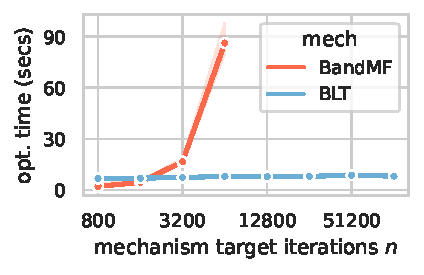
\includegraphics{images/opt_time.pdf} %
    \captionof{figure}{Total wall clock optimization time including JIT compilation on a V100 GPU for \bandmf and \blts, fixing $\minsep=400$ and varying $\nd$. The average over 3 runs is reported.}
    \label{fig:faster}
  \end{minipage}%
\end{table*}


Combining these elements gives us an efficient and differentiable algorithm for computing \maxloss and \rmsloss. Complete pseudo-code for the differentiable loss calculation is given in \cref{alg:blt_loss}. Following \citet{mcmahan2024efficient}, we use auto differentiation and L-BFGS optimizer in JAX~\citep{jax2018github} to optimize $(\theta, \hth)$ for the BLT-DP-FTRL algorithm, and then extract $\bltm(\theta, \omega)$ for noise generation. Similar to \citep{mcmahan2024efficient}, we introduce log-barrier penalties w/ strength $10^{-7}$ to keep $\omega > 0$, $\theta > 0$ and $\theta < 1$ (which is necessary to ensure the Toeplitz coefficients of $\bfC$ are decreasing to satisfy \cref{thm:toepminsepsens}).  
For high precision optimization, we use double precision in JAX on CPUs and GPUs. We observe that increasing buffer size $d$ does not necessarily reduce the loss due to numerical stability and optimization challenges, and different BLT parameter $(\theta, \omega)$ may be achieved in different optimization runs. We also highlight that the different BLT parameters $(\theta, \omega)$ can generate similar Toeplitz coefficients for $\bfC$, which suggests a smaller $d$ might help mitigate the optimization challenge from overparametrization.

The primary motivation for utilizing the $(\theta, \hth)$ parameterization in \cref{alg:blt_loss} is computational efficiency. \cref{tab:c_inv_coef} compares the time to compute $n$ Toepltiz coefficients for $\bfC\inv$ given either $\bltm(\theta, \omega)$ or given $(\theta, \hth$). In the first caes (``brute force''), we construct the Toeplitz coefficients of $\bfC$ using \cref{eq:closedcoefs}, and then solve a linear system (using \texttt{jax.lax.scan} and the property that the inverse of a lower triangular Toeplitz matrix is also lower triangular Toeplitz) to compute the coefficients of $\bfC\inv$). In the second case, we use \cref{alg:blt_pair} to compute $(\omega, \homega)$, and then compute the Toeplitz coefficients by applying \cref{eq:closedcoefs} to $\bltm(\hth, \homega)$. The comparison uses a V100 GPU and a compiled \texttt{jax} implementation, and is repeated many times with an average is given. The second approach can be fully vectorized, and is orders of magnitude faster. This is critical because this is the primary computational step in computing the \rmsloss or \maxloss and occurs in the inner loop of the mechanism optimization procedure: the net result is mechanism optimization is substantially faster than for \bandmf, and scales to much larger $\nd$, see \cref{fig:faster}. \cref{alg:blt_loss} does incur more \texttt{jax} just-in-time (JIT) compilation overhead compared to \bandmf optimization, which accounts \blt optimization being slightly slower for small $\nd$.
}{}

\ifthenelse{\boolean{acl}}{
\section{More \rmsloss and \maxloss Experiments} \label{app:mse}

\begin{figure}[H]
    \centering
    % FROM: TODO
    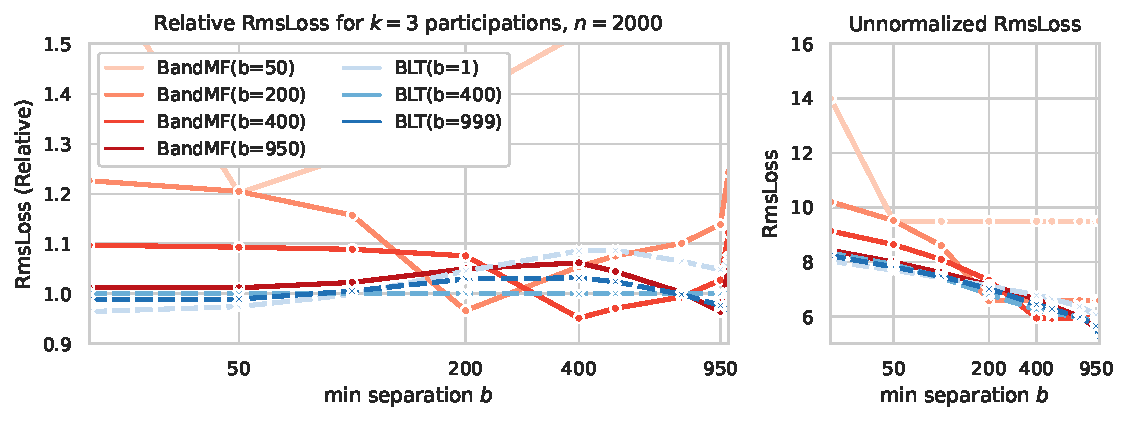
\includegraphics[width=\linewidth]{images/rmse_vary_min_sep_k3.pdf}
    \caption{Comparison of \bandmf and \blts with $\nd = 2000$ and $k=3$ participations, varying the min-separation $\minsep$. The \blts were optimized for \rmsloss. The $x$-axis is shown on a log-scale. The left panel gives loss relative to the $\bltm(b=400)$ mechanism, while the right panel gives the same data on an unnormalized $y$-axis scale.}
    \label{fig:rmse_k3}
\end{figure}

\begin{figure}[H]
    \centering
    % FROM: TODO
    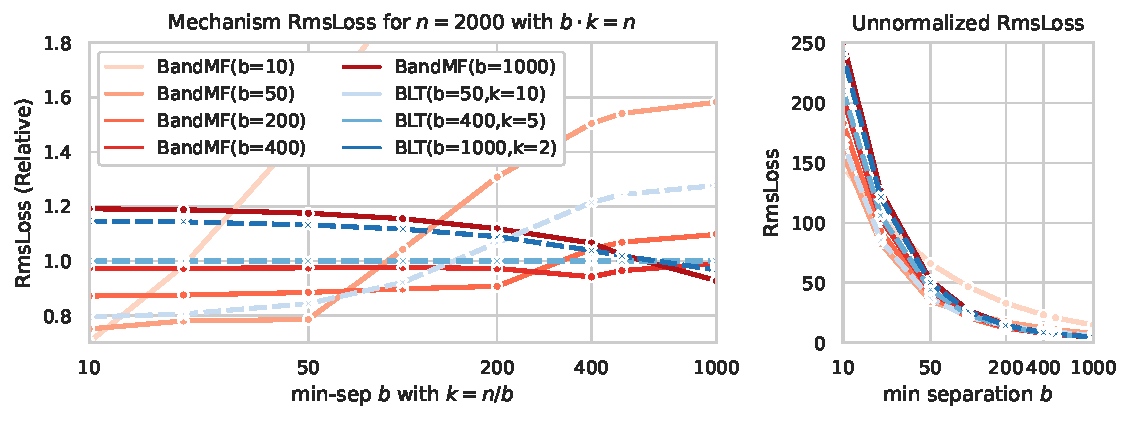
\includegraphics[width=\linewidth]{images/rmse_nkb.pdf}
    \caption{Comparison of \bandmf and \blts with $\nd = 2000$, varying $\minsep$ such that $\maxpart = \nd / \minsep$ is an integer. The \blts were optimized for \rmsloss. The $x$-axis is shown on a log-scale. The left panel gives loss relative to the $\bltm(b=400)$ mechanism, while the right panel gives the same data on an unnormalized $y$-axis scale.}
    \label{fig:rmse_nkb}
\end{figure}


\paragraph{Robustness to Min-sep $b$} \cref{fig:rmse_k3} compares BLT to the strong baseline \bandmf, fixing $\nd = 2000$ and $k=3$ participations and varying the min-separation $\minsep$. We make three primary observations: 
\begin{enumerate*}[label=\color{purple}(\arabic*)]
\item 
%The optimization of the \bandmf mechanisms does not depend on $\maxpart$, and so implicitly is designed for the case where $\maxpart \sim \nd / \minsep$ and $b \geq \hat b$; 
The optimization of the \bandmf mechanisms implicitly assumes $b \sim \hat b$, and
as expected, near this regime \bandmf in fact (slightly) outperforms the \blts. 
\item However, when $b \ll \nd / \maxpart$,  the \blts perform better. 
\item Interestingly, \bandmf performs significantly worse than the \blts at $b=999$. In this case, the only participation patterns that actually have 3 participations are e.g. $\{0, 999, 1998\}$, $\{0, 1000, 1999\}$ --- importantly, only the columns $\{0, 1, 999, 1000, 1998, 1999\}$ can ever occur in a 3-participation pattern. Because the columns of $\bfC$ for \bandmf all have the same column norm, this fact cannot be exploited. However, because of their Toeplitz structure, columns 1998 and 1999 have smaller norms than other columns, and that is beneficial in this situation. 
\end{enumerate*}

The setting where $\maxpart$ is fixed and we vary $\minsep$ includes situations that should generally be avoided in practice. For example, if we had $\maxpart=3$, $\minsep=10$, and $\nd=2000$, this indicates we had enough data we should have been able to achieve $\minsep = \nd/\maxpart \approx 667$, and so $\minsep=10$ indicates a highly suboptimal data ordering.  Similarly, if we had $\maxpart=3$, $\minsep=999$, and $\nd=2000$, then we would have been better off stopping at $n=1998$, which would have ensured only $\maxpart=2$ participations and significantly decreased sensitivity (at presumably a small cost in learning performance compared to training for $\nd=2000$ iterations).

\cref{fig:rmse_nkb} shows the contrasting scenario (indicating an essentially optimal data ordering, general not possible in federated learning) that occurs when we fix $\nd = 2000$, and choose $\minsep$ that exactly divide $\nd$ so that we can take $\maxpart = \nd / \minsep$ exactly. \cref{fig:rmse_nkb} considers the worst-case max participation $k$ for given min-sep $b$ and total rounds $n$, and achieves generally larger \rmsloss. When $b \leq \hat b$, \bandmf slightly outperforms \blts, but \bandmf degrade more rapidly for $b \leq \hat b$. In general, the curves of \blts are more smoother across different min-sep $b$ in both \cref{fig:rmse_k3} and \cref{fig:rmse_nkb}.

\paragraph{Robustness to Total Rounds $n$} \cref{fig:rmse_vary_n} considers varying the number of steps of the mechanism actually executed for mechanisms optimzied for different $\nd$. \bandmf mechanisms can only be used up to the $\nd$ they are optimized for, but \blts naturally extend to any $\nd$. This figure demonstrates that again \blts are not particularly sensitive to the $\nd$ for which they are optimized. For this figure, the maximum number of participations is chosen to be the largest allowed given $\nd$ and $\minsep=400$ (i.e., $k=n/d$), leading to the stairstep behavior of the unnormalized \rmsloss in \cref{fig:rmse_vary_n} (Right). \bandmf optimizing for large $n$ performs well when the actual number of iterations executed is small, but optimizing for large $n$ encounters nontrivial as discussed in \cref{tab:mechanism_summary} and \cref{fig:faster}. Finally, these results show that only $\nbuf=2$ buffers is sufficient for good performance, or a $200\times$ memory savings compared to \bandmf with $\minsep=400$ bands.

%\zx{We potentially want another figure to compare with \tafull, and fix a $k$ when optimizing BLTs.}

\begin{figure}[htb]
    \centering
    % FROM: TODO
    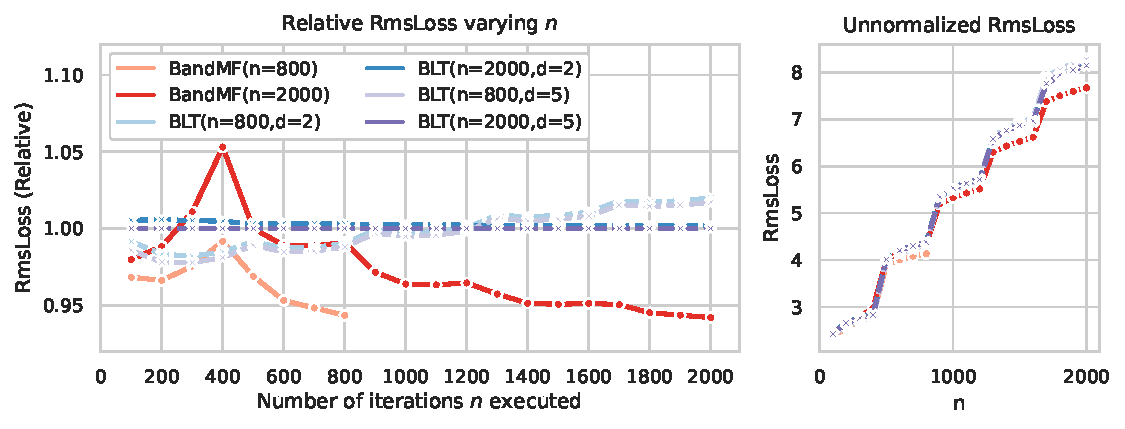
\includegraphics[width=\linewidth]{images/rmse_vary_n.pdf}
    \caption{Comparison of \bandmf and \blts optimized for $\nd=800$ and $\nd=2000$, and evaluated for $\nd$ up to the optimization target (for $\bandmf$) and over $[0, 2000]$ for the \blts. All mechanisms were optimized for min-separation (bands) $\minsep=400$. \blts with $\nbuf=2$ and $\nbuf=5$ perform almost equivalently; $\nbuf=1$ (not shown),is not sufficient with relative \rmsloss $> 1.07$.}
    \label{fig:rmse_vary_n}
\end{figure}

\begin{figure}[htb]
    \centering
    % FROM: https://colab.corp.google.com/drive/1_BRrt0jUniaOixKwasKDr7jiSToRwJLj#scrollTo=cYshzSOPA4wL&uniqifier=1
    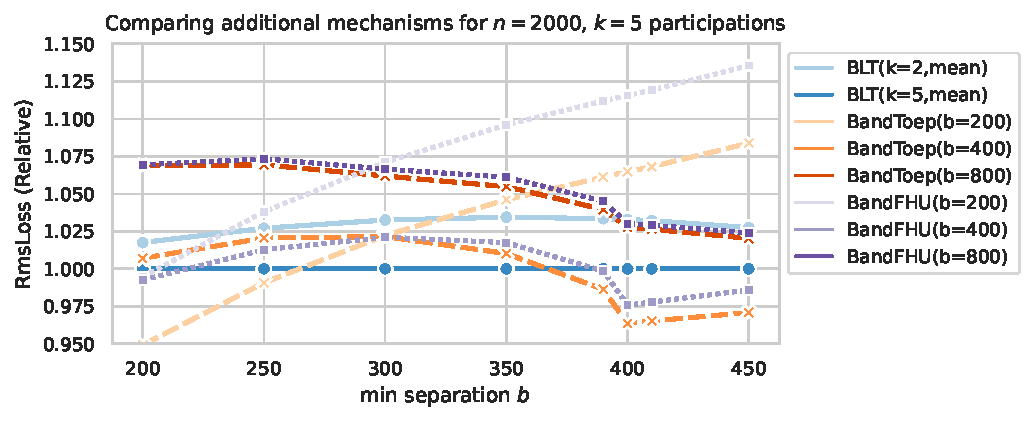
\includegraphics[width=\linewidth]{images/rmsloss_other_mechs.pdf}
    \caption{Comparison of mechanisms for $\nd=2000$ and $\maxpart=5$ participations, optimized for min-separation $\minsep = 400$ and compared for different actual values of min-separation. The setting is comparable to that of \cref{fig:rmse}, so only relative lines are given. 
    }
    \label{fig:other_mechs}
\end{figure}



\paragraph{Comparing \blt to \bandtoep and \bandfhu} Finally, we compare BLT-DP-FTRL to several other more recent mechanisms:
\begin{itemize}
    \item \bandtoep~\citep{mckenna2024scaling}, which optimizes banded Toeplitz matrices $\bfC$ for \bparticipation under \rmsloss. The primary advantage of this mechanism compared to \bandmf is that \bandtoep matrices can be optimized for much larger $\nd$. However, the runtime is the same as \bandmf, and the optimization is still slower than the optimization of \blts.
    \item \bandfhu~\citep{kalinin2024banded}, which uses prefixes of the optimal-for-single-participation \maxloss coefficients of \citet{fichtenberger2022constant} to form banded Toeplitz matrices. These will likely be worse than \bandtoep (which is specifically optimized for multiple participations), but require no mechanism optimization.
\end{itemize}
\cref{fig:other_mechs} shows that \blts are comparable or better to both of these approaches.
}{}

\section{BLT Parameters for Production Training} \label{app:blt_params}
We provide the \ourblt parameters we generated and used in training production LMs with DP FL in \cref{sec:gboard}. The \ourblt matrices are optimized for three min-sep settings $b=(100, 400, 1000)$ and each BLT is parameterized by 8 values for buffer size $d=4$, i.e., buffer decay $\theta \in \R^d$ and output scale $\omega \in \R^d$. 
\begin{itemize}
    \item min-sep $b=100$, total rounds $n=2000$, max participation $k=10  \, \Rightarrow$, \\
    $\theta=(        0.989739971007307,
        0.7352001759538236,
        0.16776199983448145,
        0.1677619998016191)$, 
        $\omega = (        0.20502892852480875,
        0.23357939425278557,
        0.03479503245420878,
        0.03479509876050538)$.
    \item min-sep $b=400$, total rounds $n=4000$, max participation $k=5  \, \Rightarrow$, \\
    $\theta=(0.9999999999921251,
        0.9944453083640997,
        0.8985923474607591,
        0.4912001418098778)$, 
        $\omega = (0.0070314825502323835,
        0.10613806907600574,
        0.1898159060327625,
        0.1966594748073734)$.
    \item min-sep $b=1000$, total rounds $n=4000$, max participation $k=2  \, \Rightarrow$, \\
    $\theta=(        0.9999999999983397,
        0.9973412136664378,
        0.9584629472313878,
        0.6581796870749317)$, 
        $\omega = (        0.008657392263671862,
        0.05890891298180163,
        0.14548176930698697,
        0.2770117005326523)$.
\end{itemize}

\cref{fig:blt_coeff} visualizes the corresponding Toeplitz coefficients for $\bfC$ to compute sensitivity and $\bfC^{-1}$ for generating correlated noise. The coefficients of $\blt(\theta, \omega)$ for $b=100$ decaying faster than $b=400$ and $b=1000$. 

\begin{figure}[thb]
\centering
\begin{subfigure}[b]{0.45\linewidth}
\centering
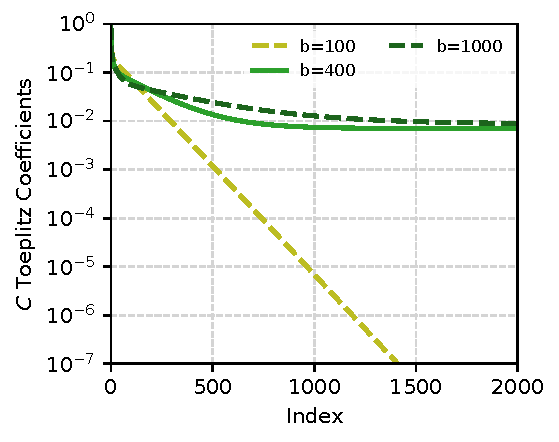
\includegraphics[width=\textwidth]{images/blt_c_coeff.pdf}
\caption{\small }
\label{fig:blt_c}
\end{subfigure}
%
\begin{subfigure}[b]{0.44\linewidth}
\centering
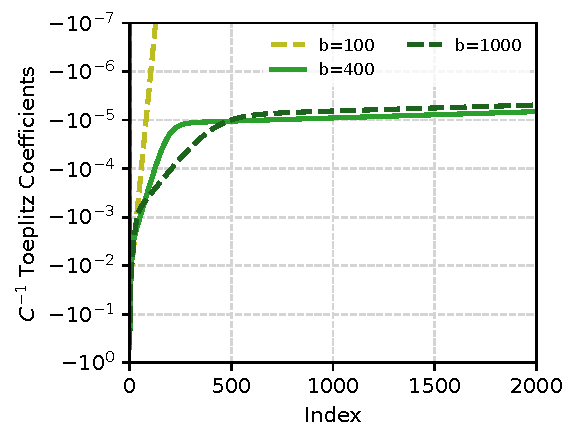
\includegraphics[width=\textwidth]{images/blt_c_inv.pdf}
\caption{\small }
\label{fig:blt_c_inv} 
\end{subfigure}
\caption{\small Toeplitz coefficients $\{c_0,\ldots,c_n\}$ for $\bfC=\LtToep(c)$ and $\{\hat c_0,\ldots,\hat c_n\}$ for $\bfC^{-1}=\LtToep(\hat c)$; For $\blt(\theta, \omega)$, $c$ can be computed by \cref{eq:closedcoefs}, and there are many ways to derive corresponding $\hat c$ (e.g., set $\bfZ=\bfI$ in \cref{alg:multCinv}).}\label{fig:blt_coeff}
\end{figure}

\section{Additional Simulation and Production Results} \label{app:plots}
\ifthenelse{\boolean{acl}}{
\subsection{Production Setting for Mobile Keyboard LMs} \label{app:prod_config}
Following \citet{hard2018gboard,xu2023federated}, we train one-layer LSTM LMs of $\sim6.4M$ parameters for mobile keyboard applications. These LMs are deployed on device to predict words during decoding time to facilitate user typing. 
We use next word prediction (NWP) accuracy on a hold-out set of devices to track the training progress, and also conduct A/B test in production, where following two metrics are reported:
\begin{enumerate*}[label=\color{purple}(\arabic*)]
    \item Word Modified Ratio (WMR), the ratio of words being modified during typing or after committed; improvement is shown by reduction;
    \item Word Per Minute (WPM): the number of committed words per minute.
\end{enumerate*}
LMs are trained for different language-locale combination in different populations. We study Spanish in Spain (es-ES), Indonesian in Indonesia (id-ID), Portuguese in Brazil (pt-BR) and Portuguese in Portugal (pt-PT). LMs are pre-trained on public multilingual C4 dataset~\citep{xue2020mt5} before private training with FL and DP. 

\paragraph{Algorithm Setting} We compare our BLT-DP-FTRL algorithm with \treeagg~\citep{kairouz21practical,xu2023federated} and \bandmf~\citep{choquette2023amplified} discussed in \cref{sec:background}. As far as we know, these two are the only DP algorithms actively used to train LMs in a production FL system. We follow the system and parameter configurations in~\citep{xu2023federated,choquette2023amplified,gboard_dp_blogpost} for baselines, and compare to \treeagg for pt-PT and id-ID, and \bandmf for es-ES and pt-BR. However, we highlight it is challenging to exactly reproduce the settings, especially for the min-sep parameter. The \bandmf algorithm are optimized for total round $n=2000$, band $\hat b = 400$ for es-ES, and $\hat b = 1000$ for pt-BR. We optimize \blt for total round $n=4000$\footnote{As the target round is usually less than 2000, $n=4000$ for \blt is less favorable compared to $n=2000$ used for \bandmf. \blt is robust to the target round $n$, and achieves stronger results with an inferior $n$.}, estimated min-sep $b=100$ for pt-PT, $b=400$ for es-ES and id-ID, and $b=1000$ for pt-BR. We use \ourblt for multi-participation and estimate the max-par based on $n/b$. For these $n,b$ settings, only $d=4$ buffers can achieve near-optimal loss in optimization, and \ourblt matrices are parameterized by only 8 numbers (these parameters are provided in \cref{app:blt_params}). Though different configures are used for populations with different sizes, the BLT parameters $(\theta, \outp) \in \R^8$ optimized for $b=400$ can achieve competitive results for a wide range of min-seps, which can be a reasonable default for BLT-DP-FTRL. As discussed in \cref{tab:mechanism_summary}, \blt is more memory-efficient than both \treeagg and \bandmf. In the simulation results \cref{tab:sonwp}, \blt is also better than \treeagg for privacy-utility trade-off, and comparable with \bandmf. The results in production further show that the flexibility of \blt makes it easier to use in practice, and achieve better results than both \treeagg and \bandmf.
\subsection{Extrapolation Results for Production Setting} \label{app:extrap}
%%%%%%%%%%%%%%%%%%%%%%%%%%%%%%%%%%%%%%%%
\begin{figure}[thb]
\centering
% 
\begin{subfigure}[b]{0.45\linewidth}
\centering
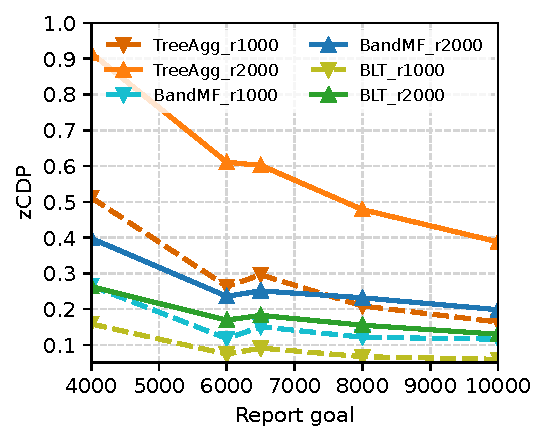
\includegraphics[width=\textwidth]{images/blt_pop3m.pdf}
\caption{\small Population 3M}
\label{fig:pop3m}
\end{subfigure}
%
\begin{subfigure}[b]{0.45\linewidth}
\centering
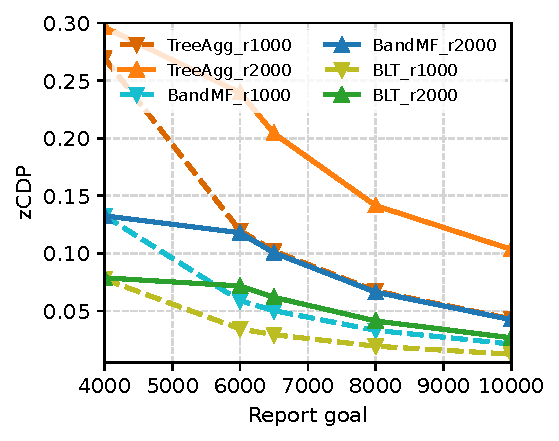
\includegraphics[width=\textwidth]{images/blt_pop10m.pdf}
\caption{\small Population 10M}
\label{fig:pop10m}
\end{subfigure}
%
\begin{subfigure}[b]{0.45\linewidth}
\centering
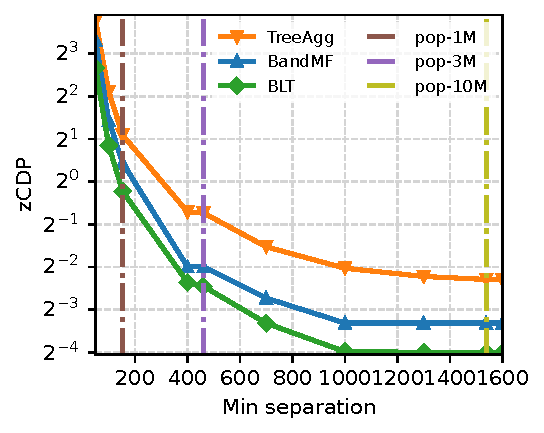
\includegraphics[width=\textwidth]{images/blt_min_sep.pdf}
\caption{\small Report goal 6500, worst-case max-par}
\label{fig:min_sep}
\end{subfigure}
%
\begin{subfigure}[b]{0.45\linewidth}
\centering
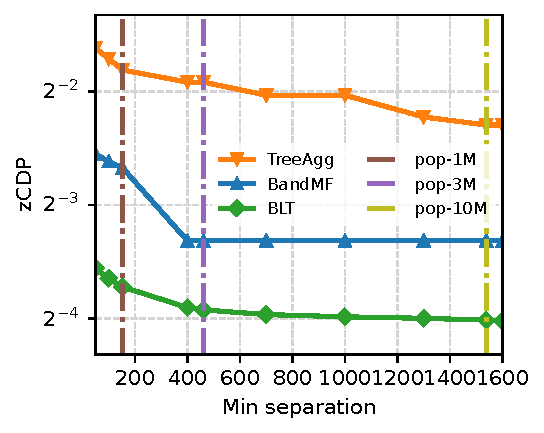
\includegraphics[width=\textwidth]{images/min_sep_max2.pdf}
\caption{\small Report goal 6500, optimistic max-par=2}
\label{fig:min_sep_max2}
\end{subfigure}
%
\caption{\small The effect of population size, number of rounds, report goals, and min-seps on DP-FTRL privacy guarantees. The results are extrapolate from the setting for es-ES and id-ID (\bandmf and \blt matrices are optimized for min-sep=400) based on the hypothesis that linearly scale noise multiplier and report goal, or only change min-sep will not affect the model utility. The For a fixed number of rounds to achieve utility target, increasing report goal and min-sep can achieve stronger guarantees measured by smaller zCDP. The optimal min-sep is capped by population size for a fixed report goal, and \blt provides better guarantees, and smoother transition across different min-seps. 
}\label{fig:extrapolate}
\end{figure}
%%%%%%%%%%%%%%%%%%%%%%%%%%%%%%%%%%%%%%%%

\paragraph{Extrapolation} We extrapolate the results for production setting by using a common hypothesis: linearly increase report goal and noise multiplier will not change the utility of the model as the signal-to-noise ratio is maintained. In addition, we assume only changing min-sep will not change the utility because of the signal-to-noise ratio. The hypothesis has been verified in previous work~\citep{kairouz21practical} and the large report goal experiments for pt-BR and pt-PT in \cref{tab:gboard} and \cref{fig:acc_curve}. Hence we can study the effect on DP without actually training the model, similar to \cref{sec:rmse_exp} for simulation.

We vary the report goal, and the min-sep is optimistically estimated by \emph{min-sep=$\lfloor$population-size/report-goal$\rfloor$}, and \emph{max-par=$\lceil$total-rounds/min-sep$\rceil$} is used unless otherwise specified. We discuss the extrapolation results in \cref{fig:extrapolate}, where utility is the same based on the hypothesis.
\begin{enumerate*}[label=\color{purple}(\arabic*)]
\item \blt achieves better DP guarantees because of its robustness to min-seps and total rounds. 
\item We observe that using larger report goal and optimizing for the largest possible min-sep achieves better results than using smaller report goals and larger corresponding min-sep, similar to observation for \treeagg in \citep{xu2023federated}.
\item \cref{fig:pop10m} shows training more rounds does not necessarily increasing DP guarantees when min-sep is large.
\item The gap of \blt and \bandmf is small when min-sep is accurately estimated. In the regime of relatively high signal-to-noise ratio (large noise multiplier for limited computation resources), \blt is competitive in a wide range of different configurations. Hence \blt is easier to use in production FL systems compared to \bandmf, and also saves memory during training.
\end{enumerate*}

Finally, in \cref{fig:varyn}, we extrapolate the DP guarantee results by varying the number of total rounds $n$ with the noise multiplier for the fixed report goal $6500$, fixed min separation $b=100,400,1000$, and corresponding max participation $k= n / b$. The \treeagg, \blt and \bandmf mechanisms used in production are compared. Instead of using \rmsloss or \maxloss to measure privacy-utility trade-offs in \cref{fig:rmse,fig:rmse_vary_n}, here we fix utility based on empirical utility of the production training and the signal-to-noise-ratio hypothesis, and compare the DP guarantees. As mentioned before, using \bandmf beyond the optimized matrices for $n=2000$ has not been studied before, and hence we only extrapolate \bandmf up to $n=2000$ rounds. \treeagg and \blt can run arbitrary number of rounds, and \blts achieve stronger DP guarantees than \treeagg. In practice, we can use one of the BLTs as a default mechanism across different settings, and perform on-the-fly optimization for given customized setting.  

\begin{figure}[thb]
\centering
\begin{subfigure}[b]{0.325\linewidth}
\centering
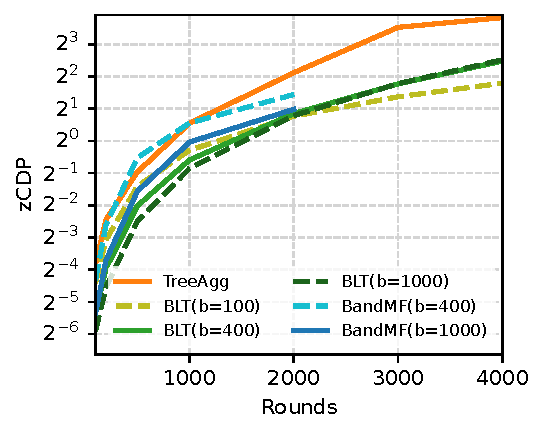
\includegraphics[width=\textwidth]{images/varyn_b100.pdf}
\caption{\small Min-sep b=100}
\label{fig:varyn_b100}
\end{subfigure}
%
\begin{subfigure}[b]{0.33\linewidth}
\centering
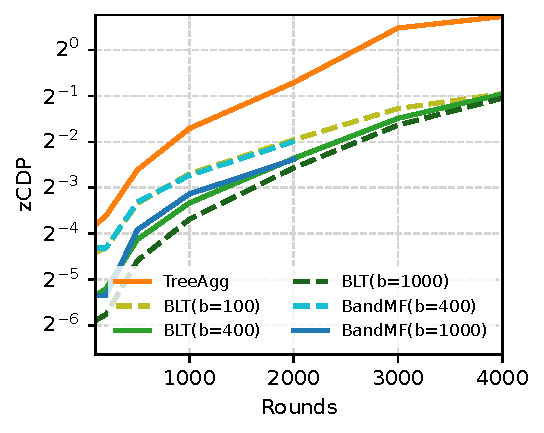
\includegraphics[width=\textwidth]{images/varyn_b400.pdf}
\caption{\small Min-sep b=400}
\label{fig:varyn_b400} 
\end{subfigure}
%
\begin{subfigure}[b]{0.33\linewidth}
\centering
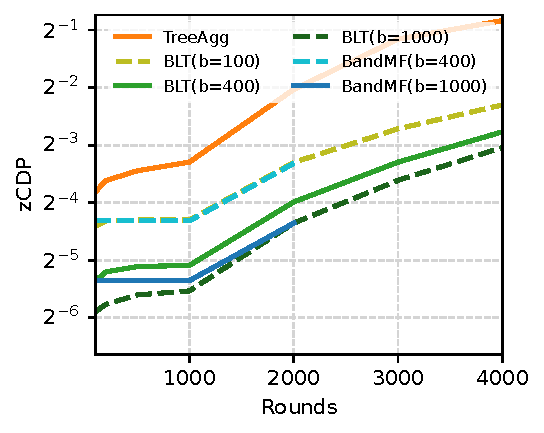
\includegraphics[width=\textwidth]{images/varyn_b1000.pdf}
\caption{\small Min-sep b=1000}
\label{fig:varyn_b1000} 
\end{subfigure}
%
\caption{\small Extrapolate by varying number of rounds $n$ for the \treeagg, \blt and \bandmf mechanisms used in production. Use the noise multiplier for the fixed report goal $6500$; fix min separation $b=100,400,1000$, respectively; worst-case max participation is varied assuming fixed population size, i.e., $k= n / b$. The utility of different mechanisms at a specific round (x-axis value) are assumed to be similar due to the signal-to-noise ratio hypothesis, and we can compare the corresponding zCDP guarantees (y-axis value).}\label{fig:varyn}
\end{figure}

\paragraph{Model launches} We have launched several language models for on-the-fly (OTF) rescoring words in Gboard smart completion and suggestion~\citep{gboard_dp_blogpost,xu2023federated}. The models trained with BLT-DP-FTRL algorithm in this paper achieved better privacy-utility trade-off than the \treeagg-DP-FTRL algorithm~\citep{kairouz21practical} widely used in FL practice~\citep{xu2023federated}, and comparable with MF-DP-FTRL~\citep{choquette2023amplified} that achieves state-of-the-art performance and some $\epsilon<1$ models reported in~\citep{gboard_dp_blogpost}. We report $\rho$-zCDP and $(\epsilon, \delta)$-DP of $\delta=10^{-10}$ following~\citet{xu2023federated,gboard_dp_blogpost}; the details of the DP configuration are provided in \cref{app:privacy-guarantees}. The Portuguese OTF LM in Brazil (pt-BR) is launched with DP $\epsilon=1.234$ (alternatively, zCDP $\rho=0.022$);
pt-PT OTF LM is launched with DP $\epsilon=8.19$ (alternatively, zCDP $\rho=0.749$) compared to DP $\epsilon=9.56$ (alternatively, zCDP $\rho=0.99$) in~\citep{xu2023federated}, and significant improvement in WMR of $-0.91\%$; 
es-ES OTF LM is launched with DP $\epsilon=4$ (alternatively, zCDP $\rho=0.202$) compared to DP $\epsilon=9.01$ (alternatively, zCDP $\rho=0.89$) in~\citep{xu2023federated}; the id-ID OTF LM using new vocabulary constructed from~\citep{gboard_fa_blogpost} is launched with DP $\epsilon=2.74$ (alternatively, zCDP $\rho=0.099$), achieving comparable utility and replacing the previous model without DP. In addition, the discussed default BLT mechanism optimized for $b=400$ and noise multiplier 7.379 is used to train and launch more models: the English LM is launched with DP $\epsilon=4.84$ (alternatively, zCDP $\rho=0.29$); the Spanish LM in Argentina is launched with DP $\epsilon=5.73$ (alternatively, zCDP $\rho=0.392$); the Spanish LM in Mexico is launched with DP $\epsilon=11.58$ (alternatively, zCDP $\rho=1.39$); the Spanish LM in other Latin America countries is launched with  DP $\epsilon=6.84$ (alternatively, zCDP $\rho=0.54$). The new Gboard OTF LMs are trained with FL and DP following the commitment in \citep{gboard_dp_blogpost,zhang2023private}. As of May 2025, all existing FL LMs have been replaced with DP FL models, fully realizing our plan in~\citep{zhang2023private}. 
\subsection{Additional Plots}
}{}

\begin{figure*}[tbh]
    \centering
    % From https://colab.corp.google.com/drive/1vaZjMTrTIPDmTTsRtc-Rm7l_LEJUqKe6#scrollTo=QzeNkbKQWHxN&uniqifier=2
    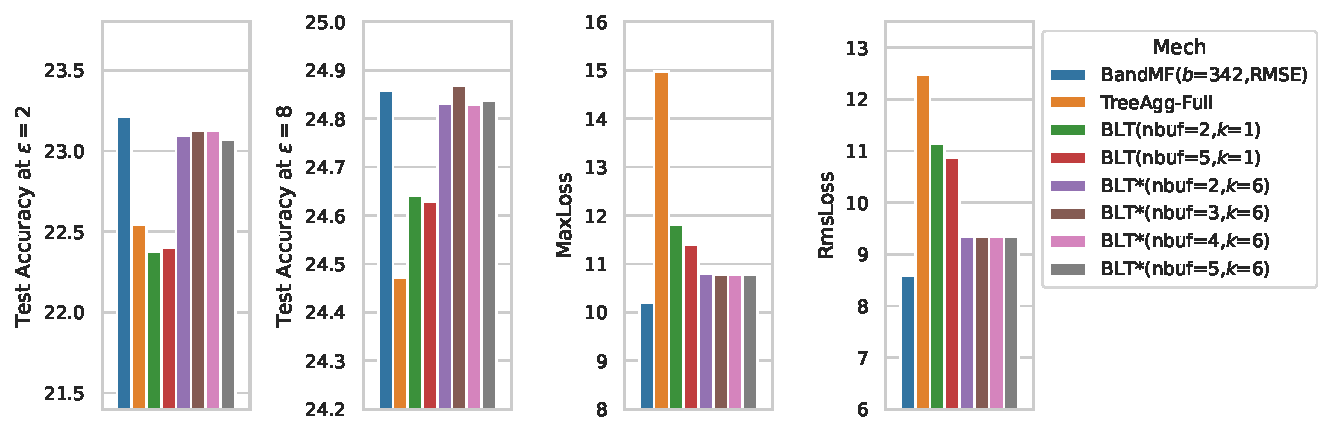
\includegraphics[width=0.8\linewidth]{images/sonwp_bar_chart.pdf}
    \caption{\small Visualizing the results in \cref{tab:sonwp}.}
    \label{fig:sonwp}
\end{figure*}

\begin{figure*}[tbh]
    \centering
    % From https://colab.corp.google.com/drive/1_BRrt0jUniaOixKwasKDr7jiSToRwJLj#scrollTo=bPzQxRSvA3rk&uniqifier=1
    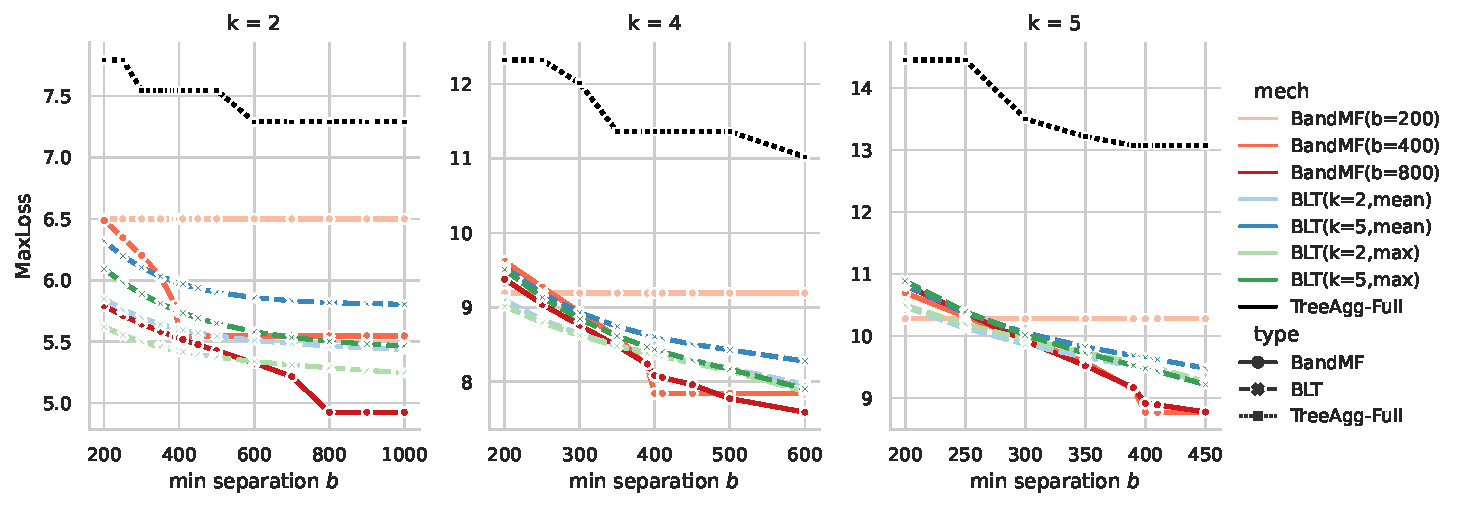
\includegraphics[width=\linewidth]{images/maxloss_k245.pdf}
    \caption{\small The same mechanisms from \cref{fig:rmse}, but compared on \maxloss instead of \rmsloss.}
    \label{fig:maxloss}
\end{figure*}

%%%%%%%%%%%%%%%%%%%%%%%%%%%%%%%%%%%%%%%%
\begin{figure*}[thb]
\centering
% 
\begin{subfigure}[b]{0.45\linewidth}
\centering
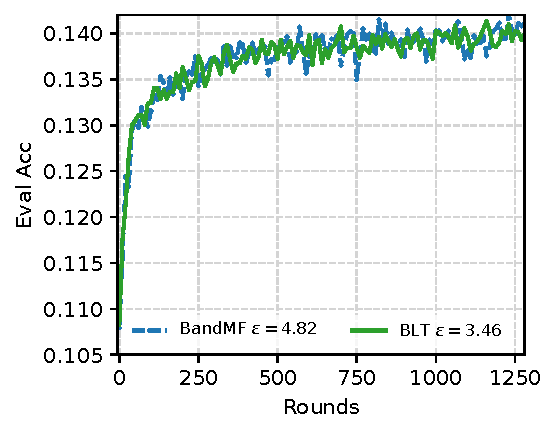
\includegraphics[width=\textwidth]{images/eses_acc.pdf}
\caption{\small Spanish LM in Spain (es-ES)}
\label{fig:es_acc}
\end{subfigure}
%
\begin{subfigure}[b]{0.45\linewidth}
\centering
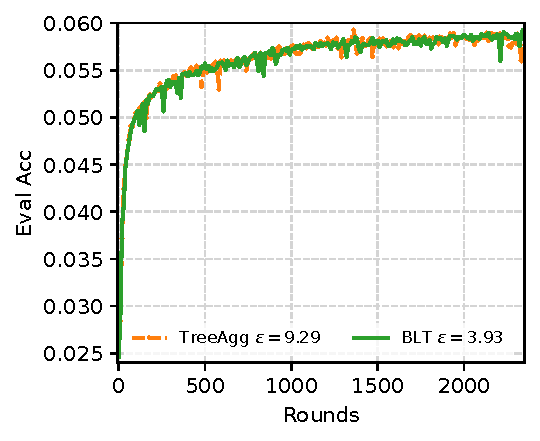
\includegraphics[width=\textwidth]{images/idid_acc.pdf}
\caption{\small Indonesian LM in Indonesia (id-ID)}
\label{fig:id_acc}
\end{subfigure}
%
\begin{subfigure}[b]{0.45\linewidth}
\centering
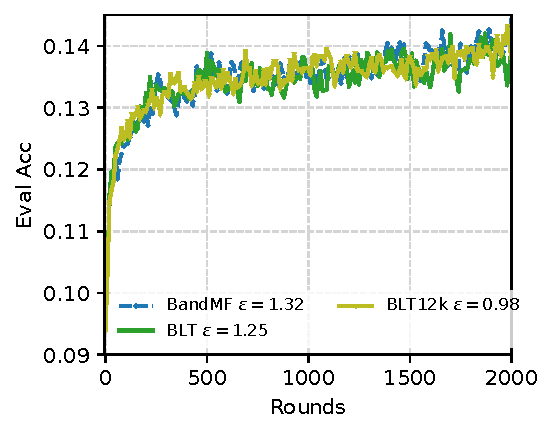
\includegraphics[width=\textwidth]{images/ptbr_acc.pdf}
\caption{\small Portuguese LM in Brazil (pt-BR)}
\label{fig:br_acc}
\end{subfigure}
%
\begin{subfigure}[b]{0.45\linewidth}
\centering
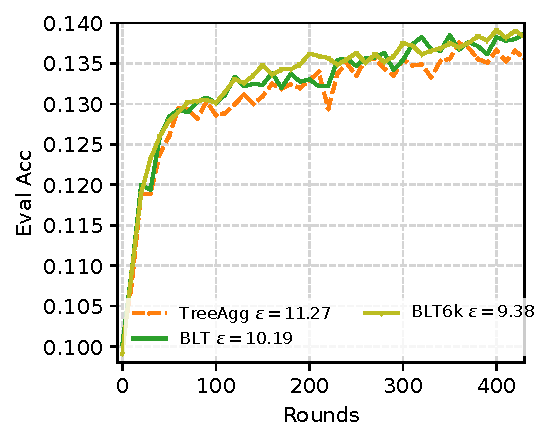
\includegraphics[width=\textwidth]{images/ptpt_acc.pdf}
\caption{\small Portuguese LM in Portugal (pt-PT)}
\label{fig:pt_acc}
\end{subfigure}
%
\caption{\small The NWP evaluation accuracy curves for training LMs with DP-FTRL in FL. \blt achieves comparable NWP accuracy and slightly better privacy guarantees (at the last round) compared to \bandmf for es-ES and pt-BR; much better DP guarantees, and/or better utility compared to \treeagg for id-ID and pt-BR.
}\label{fig:acc_curve}
\end{figure*}
%%%%%%%%%%%%%%%%%%%%%%%%%%%%%%%%%%%%%%%%
%%%%%%%%%%%%%%%%%%%%%%%%%%%%%%%%%%%%%%%%
\begin{figure*}[thb]
\centering
% 
\begin{subfigure}[b]{0.45\linewidth}
\centering
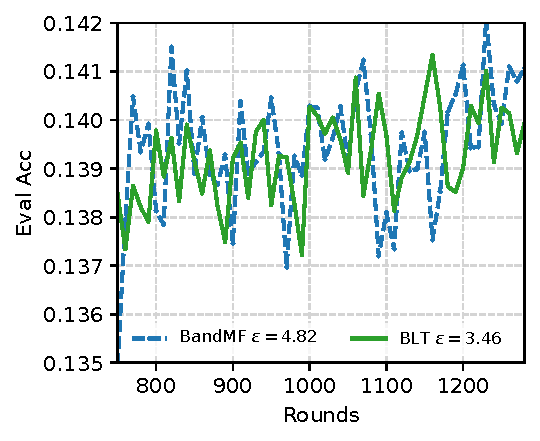
\includegraphics[width=\textwidth]{images/eses_acc2.pdf}
\caption{\small  Spanish LM in Spain (es-ES)}
\label{fig:es_acc2}
\end{subfigure}
%
\begin{subfigure}[b]{0.45\linewidth}
\centering
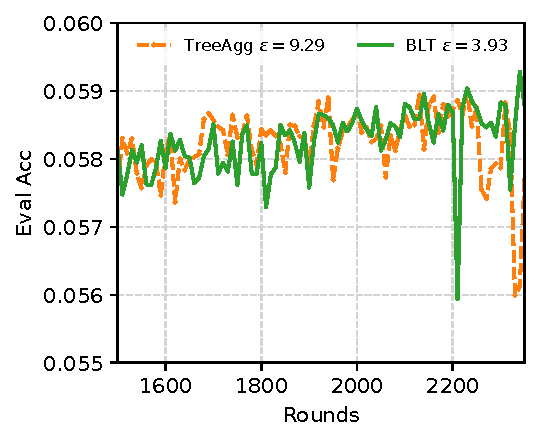
\includegraphics[width=\textwidth]{images/idid_acc2.pdf}
\caption{\small  Indonesian LM in Indonesia (id-ID)}
\label{fig:id_acc2}
\end{subfigure}
%
\begin{subfigure}[b]{0.45\linewidth}
\centering
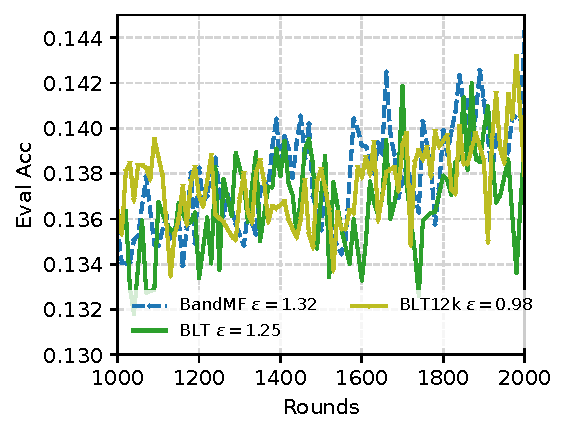
\includegraphics[width=\textwidth]{images/ptbr_acc2.pdf}
\caption{\small  Portuguese LM in Brazil (pt-BR)}
\label{fig:br_acc2}
\end{subfigure}
%
\begin{subfigure}[b]{0.45\linewidth}
\centering
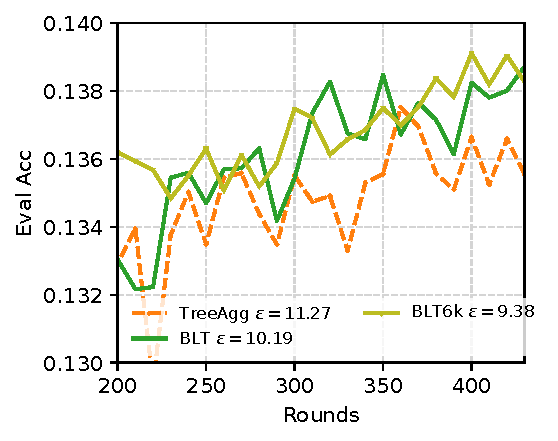
\includegraphics[width=\textwidth]{images/ptpt_acc2.pdf}
\caption{\small  Portuguese LM in Portugal (pt-PT)}
\label{fig:pt_acc2}
\end{subfigure}
%
\caption{\small  The NWP evaluation accuracy curves for training LMs with DP-FTRL in FL. Zoom in the latter stage of training for the curves in \cref{fig:acc_curve}. The NWP accuracy increases fast in the first ~200 rounds in DP FL training, and the accuracy changes within the range of $0.01$ when zooming in the later stage. The oscillation is because of the stochasticity in forming subsets of devices in both training and evaluation per round. The average NWP accuracy from nearby rounds is reported in \cref{tab:gboard} to reduce the variance. }\label{fig:acc_curve2}
\end{figure*}
%%%%%%%%%%%%%%%%%%%%%%%%%%%%%%%%%%%%%%%%
%%%%%%%%%%%%%%%%%%%%%%%%%%%%%%%%%%%%%%%%
\begin{figure*}[thb]
\centering
% 
\begin{subfigure}[b]{0.45\linewidth}
\centering
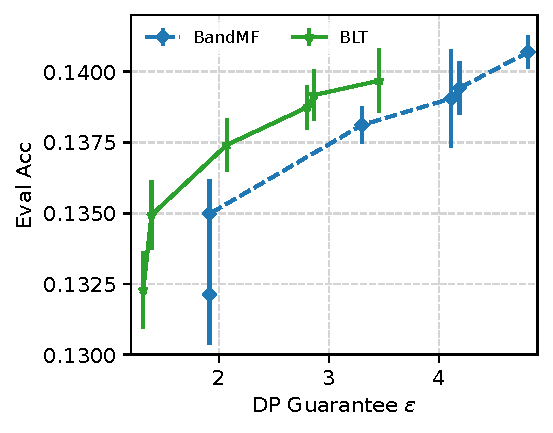
\includegraphics[width=\textwidth]{images/eses_priv.pdf}
\caption{\small Spanish LM in Spain (es-ES)}
\label{fig:es_priv}
\end{subfigure}
%
\begin{subfigure}[b]{0.45\linewidth}
\centering
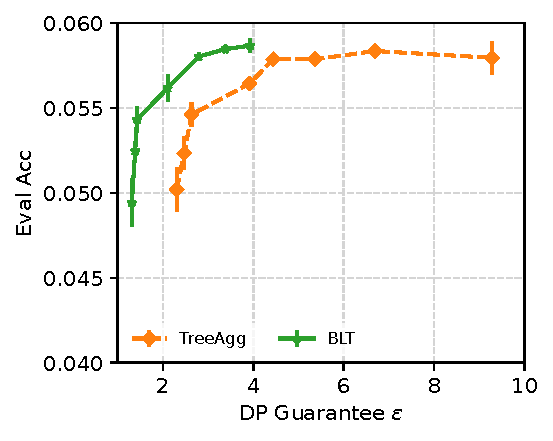
\includegraphics[width=\textwidth]{images/idid_priv.pdf}
\caption{\small Indonesian LM in Indonesia (id-ID)}
\label{fig:id_priv}
\end{subfigure}
%
\begin{subfigure}[b]{0.45\linewidth}
\centering
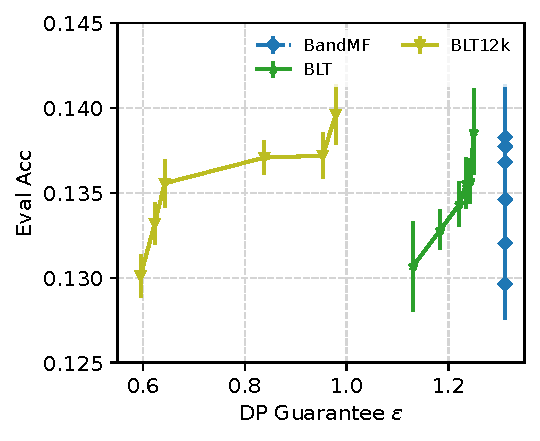
\includegraphics[width=\textwidth]{images/ptbr_priv.pdf}
\caption{\small Portuguese LM in Brazil (pt-BR)}
\label{fig:br_priv}
\end{subfigure}
%
\begin{subfigure}[b]{0.45\linewidth}
\centering
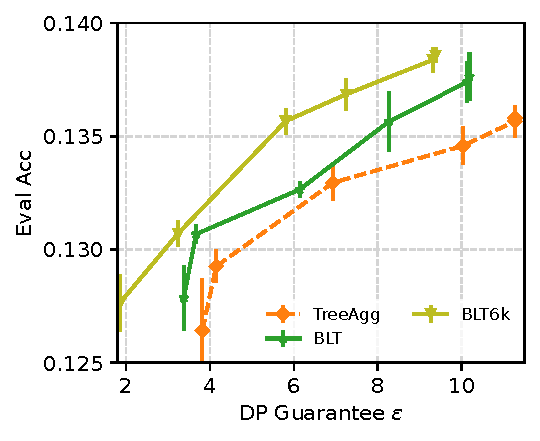
\includegraphics[width=\textwidth]{images/ptpt_priv.pdf}
\caption{\small Portuguese LM in Portugal (pt-PT)}
\label{fig:pt_priv}
\end{subfigure}
%
\caption{\small The privacy-utility trade-off curves derived from \cref{fig:acc_curve}. For each selected round $r$, we compute the mean and standard deviation (shown as vertical bars) for accuracy from the rounds in the range of $r\pm50$ ($r\pm10$ for pt-PT), and also accounting the DP guarantees. \blts show better privacy-utility trade-off as their curves are closer to the top left (small DP guarantees and large NWP accuracy).
}\label{fig:priv_curve}
\end{figure*}
%%%%%%%%%%%%%%%%%%%%%%%%%%%%%%



% \section{Proof}
% A proof is provided for completeness:
% \begin{proof}
% %\bnote{The proof currently assumes $\abs{\pi} = \maxpart$, but we need to show this. In fact, in some settings $\pistar$ might be the only participation pattern of size $\maxpart$. Probably we can address these eagerly, by arguing }
% For the proof, it will be useful to treat each $\pi$ as a list of indices given in increasing order as in \cref{eq:badpi}, rather than as a set. 
% %\[
% %  \pi = \max_{\ii \in [\maxpart]} \left\{\pi \in \arg\max_{\Pi} \norm{\bfC \ind(\pi)}, \forall i < \ii, \pi_i = \pistar_i \left\}.
% %\]
% Let $\pi \in \Pi_\minsep$ be a participation pattern that maximizes \cref{eq:sens}, and further shares a maximal-length prefix with $\pistar$ of all such optimal $\pi$. If $\pi = \pistar$, we are done. Alternatively, suppose $\pi \ne \pistar$ with $\sens(\pi) > \sens(\pistar)$. Locally, we take $\kk \coloneqq \len(\pi)$, ``lightly'' re-defining $k$ for this proof; here $k$ might be the maximum number of participations, but it could be less. Note $\pi$ cannot be a prefix of $\pistar$, because adding additional participations can only increase sensitivity in \cref{eq:sens}. Thus, there exists a minimal $\ii \in [\kk]$ such that $\pi_\ii \ne \pistar_\ii$ and by construction no other optimal $\pi$ has a smaller $\ii$; we will show a contradiction.  Let $s = \pi_\ii - \pistar_\ii \in [\nd]$, and define
% \begin{align*}
% \pi' &= (\pi_0, \pi_1, \dots, \pi_{\ii-1}, && \pi_\ii - s,&& \pi_{\ii+1} -s, \dots, \pi_\kk -s) & \\
%      &= (0, b, \dots, (\ii-1)b,            &&\ii b,  &&      \pi_{\ii+1} -s, \dots, \pi_\kk - s), &
% \end{align*}
% since by construction $\pistar_i = \pi_i$ for $i < \ii$. Essentially, we find the first opportunity to shift participations earlier, and take it. It is straightforward to verify $\pi' \in \Pi_\minsep$ as long as $\pistar$ and $\pi$ are.

% For any participation pattern $\pi$, for brevity we define 
% \[
% \sens(\pi) \coloneqq \norm{\bfC \ind(\pi)}_2.
% \]
% Then, it is sufficient to show $\sens(\pi') \ge \sens(\pi)$, a contradiction to how $\pi$ was chosen as $\pi'$ agrees with $\pi$ over a larger prefix. By definition,
% \[
% \sens^2(\pi) = \sum_{i \in [\kk]} \sum_{j \in [\kk]} \cc_{\pi_i} \cdot \cc_{\pi_j}.
% \]
% These dot products can be expressed directly in terms of the Toeplitz coefficients. Taking $a, b \in [\nd]$ with $a \le b$ wlog,
% \begin{equation} \label{eq:dotsum}
%  \cc_{\pi_a} \cdot \cc_{\pi_b} 
%   = \sum_{i=b}^n c_{i-a} c_{i-b}
%   = \sum_{i=0}^{n-b} c_{i + b -a} c_{i}.
% \end{equation}

% Matching terms in this sum between $\sens^2(\pi)$ and $\sens^2(\pi')$, we show that for all $i \in [\kk], j \in [\kk]$,
% \[
% \cc_{\pi'_i} \cdot \cc_{\pi'_j} \ge \cc_{\pi_i} \cdot \cc_{\pi_j}.
% \]
% There are four cases.
% \begin{itemize}
%   \item When $i < \ii, j < \ii$, then we have equality.
%   \item When $i < \ii, j \ge \ii$, we need to show
%   \[
%      \cc_{\pi_i} \cdot \cc_{\pi_j - s} \ge \cc_{\pi_i} \cdot \cc_{\pi_j}.
%   \]
%   This follows immediately from the fact $\cc_{\pi_i} \ge 0$ and $\cc_{\pi_j - s} \ge  \cc_{\pi_j}$ since $c$ is non-increasing.
%   \item The case $i \ge \ii, j < \ii$ is equivalent to the previous case.
%   \item When $i > \ii, j> \ii$, we need to show
%   \[
%      \cc_{\pi_i - s} \cdot \cc_{\pi_j - s} \ge \cc_{\pi_i} \cdot \cc_{\pi_j},
%   \]
%   which follows immediately from the non-negativity of $\cc$ and the rightmost expression in \cref{eq:dotsum}, which shows decreasing $a$ and $b$ by a constant simply adds more non-negative terms to the sum.
% \end{itemize}
% Thus, we conclude $\sens(\pi') \ge \sens(\pi)$, a contradiction.
% \end{proof}

\clearpage
\section{Reporting privacy guarantees}\label{app:privacy-guarantees}
This section clarifies the nuances of the DP guarantees following the guidelines outlined in \citep[Sec. 5.3]{ponomareva2023dpfy}. They are similar (if not identical)  to \citep[Appendix A]{xu2023federated} and \citep[Appendix C.3]{wu2024prompt}, except for the exact DP guarantees. We include the entire checklist for completeness.

\begin{enumerate}
    \item \textbf{DP setting}. This is a central DP guarantee where the service provider is trusted to correctly implement the mechanism.
    \item \textbf{Instantiating the DP Definition}
     \begin{enumerate}
        \item \textit{Data accesses covered}: The DP guarantee applies to all well-behaved clients\footnote{Clients that faithfully follow the algorithm including participation limits. Due to the design of the algorithm, a mis-behaved client does not adversely affect the DP guarantee of any well-behaved clients.} in a single training run. We do not account for hyperparameter tuning, or the selection of the final model checkpoint using evaluation metrics or A/B testing in our guarantees. Public data such as C4~\citep{xue2020mt5} or LLM-based synthetic data~\citep{wu2024prompt}, are used for pre-training. 
        \item \textit{Final mechanism output}: Only the final model checkpoint is released for production deployment, however the mechanism’s output is technically the full sequence of privatized gradients, and so the guarantee also applies at this level, and hence all intermediate models are protected (including those sent to devices participating in federated learning). 
        \item \textit{Unit of privacy}. Device-level DP is considered, i.e., the notion of adjacency is with respect to arbitrary training datasets on each client device, and the device might have an arbitrarily large local dataset containing arbitrary training examples. For user's with a single device, this corresponds directly to user-level DP; for devices shared with multiple users, this provides a stronger notion of DP than user-level; for a user with multiple devices that happen to both participate in training the model, the notion is weaker, but group privacy can be used to obtain a user-level guarantee.
        \item \textit{Adjacency definition for ``neigbouring'' datasets}: We use the zero-out definition~\citep{kairouz21practical}. This is a a special form of the add-or-remove definition, where neighboring data sets differ by addition/removal of a single client. In the absence of a client at any training step, we assume that the client's model update gets replaced with the all zeros vector. This assumption enforces a subtle modification to the traditional definition of the add/remove notion of DP which allows neighboring data sets to have the same number of records.
    \end{enumerate}
    \item \textbf{Privacy accounting details}
    \begin{enumerate}
        \item \textit{Type of accounting used}: Both $\rho-$zCDP~\citep{bun2016concentrated} accounting, and PLD accounting~\citep{pldlib} for $(\epsilon, \delta)-$DP are used.
        \item \textit{Accounting assumptions }: Each client only participates limited times during the training, and there are at least a min-separation number of rounds between two consecutive participation of a client. Client participation is enforced by a timer on clients in the cross-device FL system.    
        \item \textit{The formal DP statement}: See \cref{sec:gboard} \textbf{model launches} for reported DP guarantees.
        \item \textit{Transparency and verifiability}: We use the open-sourced core implementation code in TensorFlow Federated and Tensorflow Privacy. Key portions of the cross-device FL system are also open sourced.
    \end{enumerate}
\end{enumerate}